\documentclass[border=3mm,tikz,convert={outfile=jobname.svg}]{standalone}

% Colors
\usepackage{graphics}
\usepackage{xcolor}

\definecolor{darkblue}{RGB}{32, 156, 238}
\definecolor{lightblue}{RGB}{184, 223, 250}

\definecolor{darkgreen}{RGB}{34, 195, 91}
\definecolor{lightgreen}{RGB}{155, 238, 184}

% Tikz
\usepackage{tikz}
\usetikzlibrary{trees}

\tikzstyle{abstract} = [shape=rectangle, rounded corners, very thick, draw=darkblue, fill = lightblue, align=center, node distance=10cm]
\tikzstyle{concrete} = [shape=rectangle, rounded corners, very thick, draw=darkgreen, fill = lightgreen, align=center, node distance=1cm]

\begin{document}
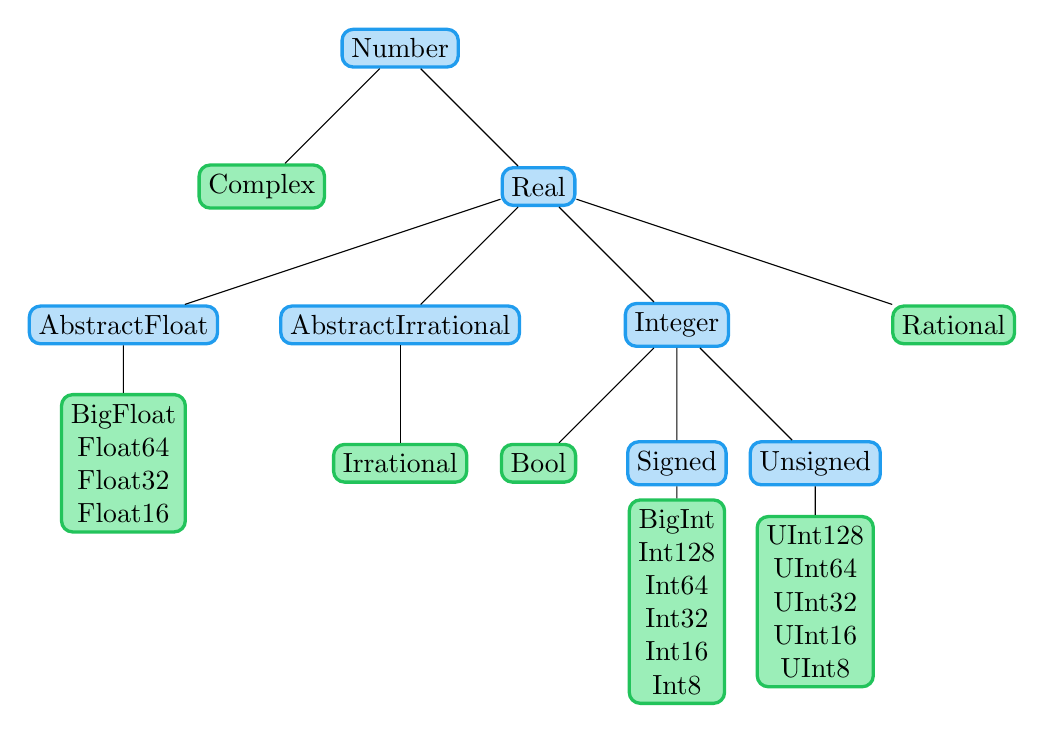
\begin{tikzpicture}[
    level distance=5em,
    level 1/.style={sibling distance=10em},
    level 2/.style={sibling distance=10em},
    level 3/.style={sibling distance=5em}
]
  \node[abstract] {Number}
    child { node[concrete] {Complex}}
    child { node[abstract] {Real}
      child { node[abstract] {AbstractFloat}
        child { node[concrete] {BigFloat \\ Float64 \\ Float32 \\ Float16}}
      }
      child { node[abstract] {AbstractIrrational}
      child { node[concrete] {Irrational}}
      }
      child { node[abstract, sibling distance = 5em] {Integer}
        child { node[concrete] {Bool}}
        child { node[abstract] {Signed}
            child { node[concrete] {BigInt \\ Int128 \\ Int64 \\ Int32 \\ Int16 \\ Int8}}
        }
        child { node[abstract] {Unsigned}
            child { node[concrete] {UInt128 \\ UInt64 \\ UInt32 \\ UInt16 \\ UInt8}}
        }
      }
      child { node[concrete] {Rational}}
    };
\end{tikzpicture}
\end{document}
